\documentclass{tufte-book} 

% setup what chapters are rendered
% This configures what chapters are rendered and what aren't
\newif\ifSpIntro
\newif\ifSpPython
\newif\ifSpComplex
\newif\ifSpSigSys
\newif\ifSpElSig
\newif\ifSpSin
\newif\ifSpFourierSer
\newif\ifSpFourierTra
\newif\ifSpDT
\newif\ifSpLTI
\newif\ifSpFResp
\newif\ifSpDTFT
\newif\ifSpFilters
\newif\ifSpUncertainty
\newif\ifSpDFT
\newif\ifSpSpectAn
\newif\ifSpFiltering
\newif\ifSpZFIR
\newif\ifSpZIIR
\newif\ifSpdB
\newif\ifSpProgA
\newif\ifSpProgB
\newif\ifSpProgC

% Comment out to disable chapter/section
% look in signal_processing.tex to see what is affected by these
% if statements
\SpIntrotrue
\SpPythontrue
\SpComplextrue
\SpSigSystrue
\SpElSigtrue
\SpSintrue
\SpdBtrue
\SpFourierSertrue
\SpFourierTratrue
\SpDTtrue
\SpLTItrue
\SpFResptrue
\SpDTFTtrue
\SpFilterstrue
\SpUncertaintytrue
\SpDFTtrue
\SpSpectAntrue
\SpFilteringtrue
\SpZFIRtrue
\SpZIIRtrue
\SpProgAtrue
\SpProgBtrue
\SpProgCtrue


% all the settings are here
\usepackage[english]{babel}
\usepackage[utf8x]{inputenc}
\usepackage[T1]{fontenc}
%% Sets page size and margins
%\usepackage[a4paper,top=3cm,bottom=2cm,left=3cm,right=3cm,marginparwidth=1.75cm]{geometry}

%% Useful packages
\usepackage{amsmath,amssymb,amsthm}
\usepackage{physics}
\usepackage{mathtools}
\usepackage{tikz}
\usepackage{pgfplots}
\usepackage{graphicx}
\usepackage{xcolor}
\usepackage{tabularx}

\usepackage[colorinlistoftodos]{todonotes}

%\usetikzlibrary{backgrounds,calc}

\usetikzlibrary{shapes,arrows,backgrounds,calc}
\usepackage{color}
\usepackage{listings}
\usepackage{bm}
\usepackage{microtype} % Improves character and word spacing
\usepackage{lipsum} % Inserts dummy text
\usepackage{booktabs} % Better horizontal rules in tables
\usepackage{graphicx} % Needed to insert images into the document
\usepackage{tabularx}
\usepackage{cancel}
\definecolor{codegreen}{rgb}{0,0.6,0}
\definecolor{codegray}{rgb}{0.5,0.5,0.5}
\definecolor{codepurple}{rgb}{0.58,0,0.82}
%\definecolor{backcolour}{rgb}{0.95,0.95,0.92}
%\definecolor{backcolour}{rgb}{0.5,0.5,0.5}
%\definecolor{backcolour}{rgb}{1.0,0.937,0.859}
\definecolor{backcolour}{rgb}{1.0,1.0,1.0}
\definecolor{skyblue1}{rgb}{0.447,0.624,0.812}
\definecolor{scarletred1}{rgb}{0.937,0.561,0.561}
\definecolor{juhagray}{rgb}{0.75,0.75,0.75}
%\definecolor{backcolour}{rgb}{1.0,1.0,1.0}
 
\lstdefinestyle{mystyle}{
    backgroundcolor=\color{backcolour},   
    commentstyle=\color{codegreen},
    keywordstyle=\color{magenta},
    numberstyle=\tiny\color{codegray}, 
    stringstyle=\color{codepurple},
    basicstyle=\footnotesize,
    breakatwhitespace=false,
    frame=shadowbox,
    rulesepcolor=\color{juhagray},
    breaklines=true,                 
    captionpos=b,                    
    keepspaces=true,                 
    numbers=none,                    
    numbersep=5pt,                  
    showspaces=false,                
    showstringspaces=false,
    showtabs=false,                  
    tabsize=2
}
 
\lstset{style=mystyle}

\usepackage[american,siunitx]{circuitikz}
\usetikzlibrary{arrows,calc,positioning}


\newcommand{\Hee}{\mathcal{H}(e^{i\hat{\omega}})}
\newcommand{\Hez}{\mathcal{H}(z)}
\newcommand{\Hew}{\mathcal{H}(\omega)} 
\newcommand{\Hec}{\mathcal{H}^*\left(e^{i\hat{\omega}}\right)} 
\newcommand{\Hem}{\mathcal{H}\left(e^{-i\hat{\omega}}\right)}
%\newcommand{\He}{\mathcal{H}\left(e^{i\hat{\omega}}\right)}

\newcommand{\He}{\mathcal{H}\left(\hat{\omega}\right)}
\newcommand{\Xe}{X\left(e^{i\hat{\omega}}\right)}
\newcommand{\Xec}{X^*\left(e^{i\hat{\omega}}\right)}
%\newcommand{\Hec}{\mathcal{H}^*\left(e^{i\hat{\omega}}\right)} 
%\newcommand{\Hem}{\mathcal{H}\left(e^{-i\hat{\omega}}\right)} 
\newcommand{\Xem}{X\left(e^{-i\hat{\omega}}\right)} 

\newcommand{\mixer}[1] 
{  % #1 = name , 
\draw[thick] (#1) circle (12pt);
\draw[rotate=45,line width=0.5pt]   (#1)  +(0,-12pt) -- +(0,12pt);
\draw[rotate=-45,line width=0.5pt]  (#1)  +(0,-12pt) -- +(0,12pt);
}
\newcommand{\BPF}[2] 
{  % #1 = name , #2 = rotation angle
\begin{scope}[transform shape,rotate=#2]
\draw[thick] (#1)node[](a){} +(-12pt,-12pt) rectangle +(12pt,12pt);
\draw (a) +(-8pt,0) to[bend left] +(0,0) edge[bend right] +(8pt,0);
\draw ([yshift=5pt]a) +(-8pt,0) to[bend left] +(0,0) to[bend right] +(8pt,0);
\draw ([yshift=-5pt]a) +(-8pt,0) to[bend left] +(0,0) edge[bend right] +(8pt,0);
\draw[rotate=20] ([yshift=5pt]a) +(-4pt,0) -- +(7pt,0);
\draw[rotate=20] ([yshift=-5pt]a) +(-7pt,0) -- +(4pt,0);
\end{scope}
}
\newcommand{\LPF}[2] 
{  % #1 = name , #2 = rotation angle
\begin{scope}[transform shape,rotate=#2]
\draw[thick] (#1)node[](a) {\footnotesize{$\mathcal{H}(\omega)$}} +(-12pt,-12pt) rectangle +(12pt,12pt);
\end{scope}
}

\newcommand{\hangp}[1]{\makebox[0pt][r]{(}#1\makebox[0pt][l]{)}} % New command to create parentheses around text in tables which take up no horizontal space - this improves column spacing
\newcommand{\hangstar}{\makebox[0pt][l]{*}} % New command to create asterisks in tables which take up no horizontal space - this improves column spacing

\tikzset{ar/.style={-latex,shorten >=-1pt, shorten <=-1pt}}
\usetikzlibrary{shapes,arrows}


\hypersetup{colorlinks} % Comment this line if you don't wish to have colored links


\setkeys{Gin}{width=\linewidth,totalheight=\textheight,keepaspectratio} % Improves figure scaling

\usepackage{fancyvrb} % Allows customization of verbatim environments
\fvset{fontsize=\normalsize} % The font size of all verbatim text can be changed here


\usepackage{xspace} % Used for printing a trailing space better than using a tilde (~) using the \xspace command

\newcommand{\monthyear}{\ifcase\month\or January\or February\or March\or April\or May\or June\or July\or August\or September\or October\or November\or December\fi\space\number\year} % A command to print the current month and year

\newcommand{\openepigraph}[2]{ % This block sets up a command for printing an epigraph with 2 arguments - the quote and the author
\begin{fullwidth}
\sffamily\large
\begin{doublespace}
\noindent\allcaps{#1}\\ % The quote
\noindent\allcaps{#2} % The author
\end{doublespace}
\end{fullwidth}
}
\usetikzlibrary{shapes,snakes}

\newcommand\Hiw{\mathcal{H}(\omega)}

\tikzset{%
    dimen/.style={|-|,>=latex,thin,every rectangle node/.style={fill=white,midway,font=\sffamily}},
}

\pgfplotsset{
    dirac/.style={
        mark=triangle*,
        mark options={scale=2},
        ycomb,
        scatter,
        visualization depends on={y/abs(y)-1 \as \sign},
        scatter/@pre marker code/.code={\scope[rotate=90*\sign,yshift=-2pt]}
    }
}

\tikzstyle{int}=[draw, minimum size=2em]
\tikzstyle{init} = [pin edge={to-,thin,black}]

 
\newcommand{\spop}[1][\cdot]{\mathcal{T}\left\{#1\right\}}
\newcommand{\spopb}{\mathcal{T}}

\newcommand{\blankpage}{\newpage\hbox{}\thispagestyle{empty}\newpage} % Command to insert a blank page

\usepackage{imakeidx} % Used to generate the index
\usepackage{hyperref}
\makeindex % Generate the index which is printed at the end of the document

%----------------------------------------------------------------------------------------
%	BOOK META-INFORMATION
%----------------------------------------------------------------------------------------
\author{Juha Vierinen} % Author
\publisher{University of Troms\o{}} % Publisher

%----------------------------------------------------------------------------------------


\newsavebox{\titleimage}
\savebox{\titleimage}{
\centering{
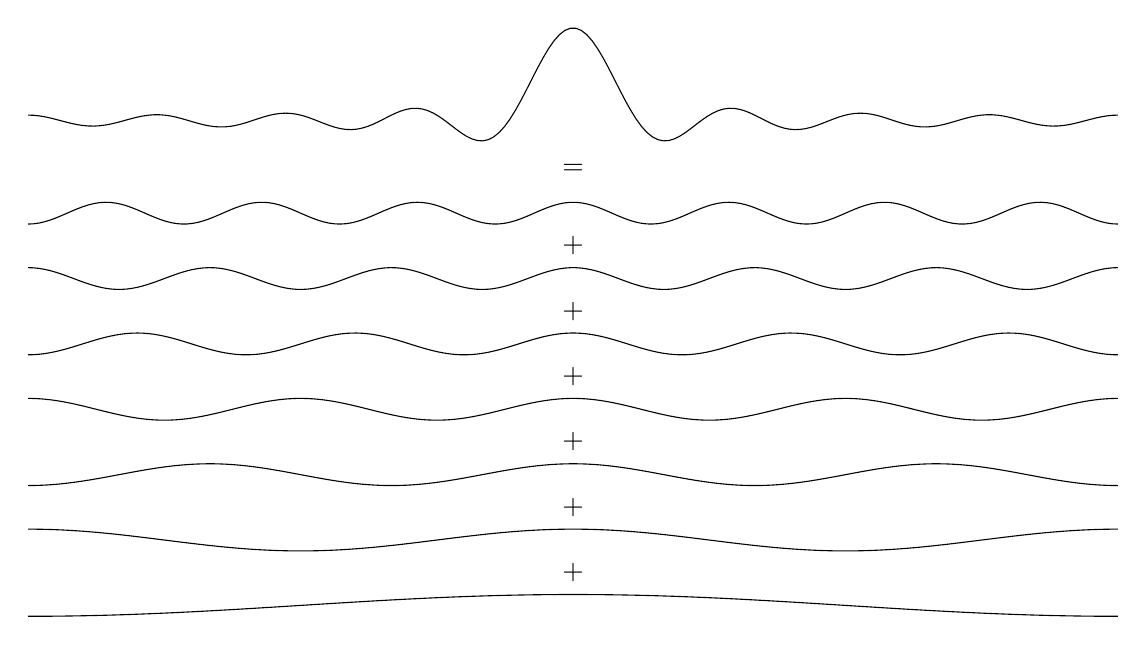
\begin{tikzpicture}
% \begin{pgfinterruptboundingbox}
\begin{axis}[width=1.5\textwidth, height=30em,
%	title={Discrete-time signal},
	axis x line=none,
	axis y line=none
]
\addplot[domain=-100:100,samples=200] {27+
                                       cos( deg(2*3.1415*0.01*0.5*x))+
                                       cos( deg(2*3.1415*0.01*0.5*2*x) )+
                                       cos( deg(2*3.1415*0.01*0.5*3*x) )+
                                       cos( deg(2*3.1415*0.01*0.5*4*x) )+
                                       cos( deg(2*3.1415*0.01*0.5*5*x) )+
                                       cos( deg(2*3.1415*0.01*0.5*6*x) )+
                                       cos( deg(2*3.1415*0.01*0.5*7*x) )+
                                       cos( deg(2*3.1415*0.01*0.5*8*x) ) };

\node at (axis cs:0,22) {$=$};
\node at (axis cs:0,15) {$+$};
\node at (axis cs:0,9) {$+$};
\node at (axis cs:0,3) {$+$};
\node at (axis cs:0,-3) {$+$};
\node at (axis cs:0,-9) {$+$};
\node at (axis cs:0,-15) {$+$};
                                      
\addplot[domain=-100:100,samples=200] {-18+cos( deg(2*3.1415*0.01*0.5*x) ) };
\addplot[domain=-100:100,samples=200] {-12+cos( deg(2*3.1415*0.01*0.5*2*x) ) };
\addplot[domain=-100:100,samples=200] {-6+cos( deg(2*3.1415*0.01*0.5*3*x) ) };
\addplot[domain=-100:100,samples=200] {0+cos( deg(2*3.1415*0.01*0.5*4*x) ) };
\addplot[domain=-100:100,samples=200] {6+cos( deg(2*3.1415*0.01*0.5*5*x) ) };
\addplot[domain=-100:100,samples=200] {12+cos( deg(2*3.1415*0.01*0.5*6*x) ) };
\addplot[domain=-100:100,samples=200] {18+cos( deg(2*3.1415*0.01*0.5*7*x) ) };
\end{axis}
%\end{pgfinterruptboundingbox}
%\draw[use as bounding box] ([xshift=0cm,yshift=0cm]current axis.south west) 
%    rectangle ([xshift=0cm,yshift=0cm]current axis.north east);
\end{tikzpicture}
}
}

\title[Signal processing]{%
  \setlength{\parindent}{0pt}%
  Signal processing\par \vspace{1cm}
    \usebox{\titleimage}
  }
  
\author{Juha Vierinen, J\o{}rn Olav Jensen}
\date{Fall 2022}


\begin{document}
\frontmatter
%----------------------------------------------------------------------------------------
%	EPIGRAPH
%----------------------------------------------------------------------------------------

%----------------------------------------------------------------------------------------

\maketitle % Print the title page

%----------------------------------------------------------------------------------------
%	COPYRIGHT PAGE
%----------------------------------------------------------------------------------------

\newpage
\begin{fullwidth}
~\vfill
\thispagestyle{empty}
\setlength{\parindent}{0pt}
\setlength{\parskip}{\baselineskip}
Copyright \copyright\ \the\year\ \thanklessauthor

\par\smallcaps{Published as lecture notes.}% \thanklesspublisher}

\par\smallcaps{\url{http://kaira.uit.no/fys2006}}

%\par License information.\index{license}

\par\textit{\monthyear}
\end{fullwidth}

%----------------------------------------------------------------------------------------

\tableofcontents % Print the table of contents

%----------------------------------------------------------------------------------------

%\listoffigures % Print a list of figures

%----------------------------------------------------------------------------------------

%\listoftables % Print a list of tables

%\lstlistoflistings

%----------------------------------------------------------------------------------------
%	DEDICATION PAGE
%----------------------------------------------------------------------------------------

%\if 0
\cleardoublepage
~\vfill
\begin{doublespace}
\noindent\fontsize{10}{10}\selectfont\itshape
\nohyphenation
I'd like to thank the following people\sidenote{or their aliases, as
some may have not chosen to use their real name when participating in
the course commentary on Perusall.} for corrections and suggestions
that have improved these lecture notes over the years: Björn
Gustavsson, Patrick Guio,
%(2020)
Mikkel Isak Gaup, Adrian Sletten,
Rikke Bjarnesen Andresen, Jostein Henriksen, Daniel Nordajl Jørgensen,
Ivan Mikheev, Oskar Marthinussen, Iver Martinsen, Marit Breimo, Sigurd
Haugse, Ragnar Helgaas, Sondre Thomassen, Sofie Svenøe, Sigurd Yngvar
Ekern, Vetle Hofsøy-Woie, Øyvind Alexander Larssen, Erlend
Thorkildsen, Amalie Gjelsvik, Tommy Ryan, Eivind Dragset, Attiqa
Abrar, Daniel Breiland Teigen, Sigrid Holm, Åse Fauske, Yvonne
Johansen, Frank Martin Fossland, Runar Folke-Olsen, Morten Paulsen,
Teodor Skotnes,
%(2021)
Martin Stave, Kristine Rein, Anna Odh, Vegar
Einarsen, Christian Salomonsen, Jonas Riise, Jørn Jensen, Anton
Zyranov, Nikolai Anfeltmo, Håkon Johansen, Kian Sadeghi, Johannes
Bjørnhaug, Ines Seeliger, Dana King, Emil Jettli, Sigurd Hanssen, Liza
Liz, Sebastian Iversen, Daniel Johansen, Tobias W. Tobiassen, and
Johanna Mankova Buseth. I'd also like to thank countless others whose
names I have forgot to mention. All mistakes are purely mine.
\end{doublespace}
\vfill
\vfill
%\fi





\cleardoublepage


%----------------------------------------------------------------------------------------
%	This is where the bulk of the content is
%       Use \if 0 and \fi to comment out the parts that you don't need to compile
%----------------------------------------------------------------------------------------
\ifSpIntro
  \chapter{Introduction}
  
\newthought{Many aspects of the life of a modern human} depend on the theory of
\index{signal processing}{signal processing}. Here are a few examples. When
you are listening to a digital audio recording of music, displaying an
image on your computer, or using a wireless internet connection, you
are relying on mathematical concepts that are taught in a basic course
on signal processing. These same concepts are encountered when e.g.,
solving differential equations, applying deep learning techniques,
measuring the gravitational wave signature of colliding neutron stars
with a laser interferometer, or making an image of a black hole using
a world wide network of radio telescopes. The theory
of \emph{\index{signals and systems}{signals and systems}} is a
collection of applied mathematical tools that have important
applications in science, technology, and engineering. The term signal
processing and the terminology of signal processing have origins in
electrical engineering.

\begin{marginfigure}[-4.2cm]
\begin{center}
\includegraphics[width=\textwidth]{ch01/figures/prism.png}
\end{center}
\caption{Light can be viewed as a superposition of electromagnetic waves
with different amplitudes, phases, and frequencies. This can be
investigated in practice with the help of a prism or a diffraction
grating. My hope is that after taking this course, you will
metaphorically be able to ``see'' arbitrary signals as a sum of
periodic harmonic functions or \emph{spectral components}.}
\label{fig:prism}
\end{marginfigure}

\newthought{Let's look more closely at the audio example}. When you
listen to a recording of music, you are probably relying on a digital
representation of the acoustic signal that
is \emph{\index{compression}{compressed}}. With the help of signal
processing mathematics, the audio signal is encoded in a special way,
which allows the size of the file to be greatly reduced. This lowers
the minimum internet speed required to stream the audio without
annoying interruptions and allows 10 to 100 times more audio files to
be stored on a digital storage device than without compression.

\index{compression algorithm}{Audio compression algorithms}
often rely on the fact that the \emph{frequency domain}
or \emph{spectral} representation of a signal is far more sparse than
the time domain representation. This means that we can approximate the
original audio signal using a sum of a relatively small number of
periodic sinusoidal signal components. Let's say that the original
audio signal is $x(t)$, which represents air pressure as a function of
time. Using the \index{Fourier series}{Fourier series} we can use the
following type of a sum to approximate $x(t)$:
\begin{equation}
x(t) \approx \sum_{n=1}^{N} A_n \sin(\omega_n t + \phi_n) \,\,,
\label{ch01:eq:fourier_ser}
\end{equation}
with each sinusoidal signal only described by three parameters: an
amplitude $A_n \in \mathbb{R}$, a phase $\phi_n \in \mathbb{R}$, and an angular frequency $\omega_n \in \mathbb{R}$.

\begin{marginfigure}
\begin{center}
  \includegraphics[width=\textwidth]{ch01/figures/euler.jpg}
\end{center}
\caption{Leonhard Euler. Credit: Jakob Handmann (1753)}
\label{fig:euler_pic}
\end{marginfigure}

If the value of $N$ in Equation \ref{ch01:eq:fourier_ser} is
sufficiently small, then the amount of information required to
represent the audio signal as a sum of sinusoids can be significantly
less than what would be required if the signal was just sampled with a
fixed sample spacing and the amplitude of the waveform at each sampled
point would be stored.

Here's an example. Let's say that you want to store 1024 \emph{samples}\sidenote{One sample is a number representing the audio signal amplitude at one instant of time} of
audio signal. With the signal represented using 44100 samples per second,
this would be approximately 0.023 seconds of signal. You'd need to
store 1024 numbers without compression. With 16 bits per sample, this
audio signal would require 16384 bits of storage space. However, if
the signal is sufficiently well represented using $N=10$ sinusoidal
components, you'd only need to store 30 numbers to retain the
information about the phase, amplitude and frequency of each
sinusoidal component. This is only approximately 3\% of the original
data, or 480 bits of storage space at 16 bits per number\sidenote{One
"bit" of information is an answer to a yes or no question. One bit
would allow you to say that a number is either 0 or 1. A two bit
signal would allow you to say that a number is either 0, 1, 2, or 3.}.

Most of the videos, images, and music that you access over the
internet is compressed in this manner. Without spectral compression
techniques, the internet would most likely need to have at least 10
times more capacity than it currently has, in order to be able to
provide us with the same amount of entertainment. For example,
the \index{MP3}{MP3} audio compression standard and
the \index{JPEG}{JPEG} image compression standard both utilize spectral
compression methods.

%This is also the reason why sometimes the audio
%in an online meeting sounds a bit ``robotic'' when you have a very
%poor internet connection -- it is represented with only a small number
%of sinusoidal components. 

\newthought{We often use more general complex valued sinusoidal functions} instead of real valued ones when describing the theory of signal
processing. These are defined as follows:
\begin{equation}
A e^{i\phi }e^{i\omega t} = A[\cos(\omega t+\phi) + i\sin(\omega
t+\phi)] \,\,.
\label{ch01:eq:euler}
\end{equation}
Just like a real valued sinusoid, the complex sinusoid is also
represented using an amplitude $A \in \mathbb{R}$, phase
$\phi \in \mathbb{R}$, and angular frequency $\omega \in \mathbb{R}$. Note
that the above equation is just an application of Euler's
formula\sidenote[][1cm]{The famous physicist \index{Richard
Feynman}{Richard Feynman} had this to say about \index{Euler's
formula}{Euler's formula}: ``We summarize with this, the most
remarkable formula in mathematics. This is our jewel.'' (Feynman
Lectures on Physics, Vol I). He had clearly benefited greatly from
this formula.}, which is probably the most frequently occurring
equation in signal processing. If you master this equation, you'll
have covered already most of this course!

If you are not familiar with complex algebra,
Equation \ref{ch01:eq:euler} might at first seem intractable. But
don't worry. If you have a hard time grasping the function $A e^{i\phi
}e^{i\omega t}$, just think of it as a periodic function like
$A\cos(\omega t + \phi)$, but with a real and imaginary sinusoidal
component. The reason for using the complex sinusoidal signal instead
of the real valued one is that most of the mathematical calculations
are greatly simplified.

\begin{marginfigure}
\begin{center}
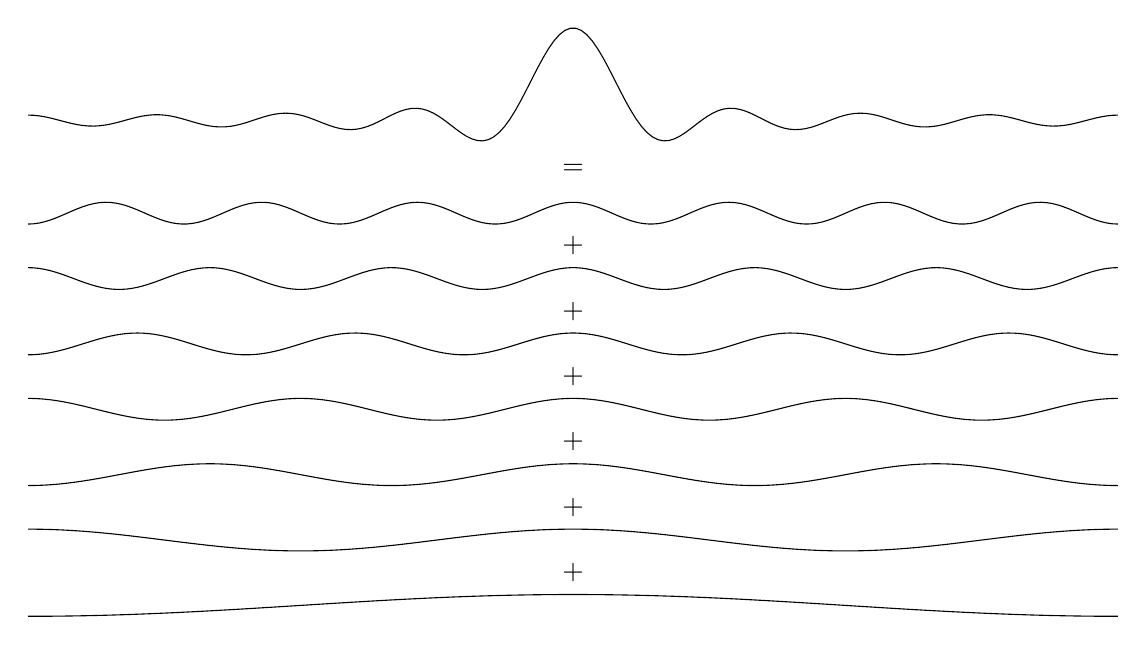
\begin{tikzpicture}
% \begin{pgfinterruptboundingbox}
\begin{axis}[width=1.5\textwidth, height=30em,
%	title={Discrete-time signal},
axis x line=none,
axis y line=none
]
\addplot[domain=-100:100,samples=200] {27+
cos( deg(2*3.1415*0.01*0.5*x))+
cos( deg(2*3.1415*0.01*0.5*2*x) )+
cos( deg(2*3.1415*0.01*0.5*3*x) )+
cos( deg(2*3.1415*0.01*0.5*4*x) )+
cos( deg(2*3.1415*0.01*0.5*5*x) )+
cos( deg(2*3.1415*0.01*0.5*6*x) )+
cos( deg(2*3.1415*0.01*0.5*7*x) )+
cos( deg(2*3.1415*0.01*0.5*8*x) ) };

\node at (axis cs:0,22) {$=$};
\node at (axis cs:0,15) {$+$};
\node at (axis cs:0,9) {$+$};
\node at (axis cs:0,3) {$+$};
\node at (axis cs:0,-3) {$+$};
\node at (axis cs:0,-9) {$+$};
\node at (axis cs:0,-15) {$+$};

\addplot[domain=-100:100,samples=200] {-18+cos( deg(2*3.1415*0.01*0.5*x) ) };
\addplot[domain=-100:100,samples=200] {-12+cos( deg(2*3.1415*0.01*0.5*2*x) ) };
\addplot[domain=-100:100,samples=200] {-6+cos( deg(2*3.1415*0.01*0.5*3*x) ) };
\addplot[domain=-100:100,samples=200] {0+cos( deg(2*3.1415*0.01*0.5*4*x) ) };
\addplot[domain=-100:100,samples=200] {6+cos( deg(2*3.1415*0.01*0.5*5*x) ) };
\addplot[domain=-100:100,samples=200] {12+cos( deg(2*3.1415*0.01*0.5*6*x) ) };
\addplot[domain=-100:100,samples=200] {18+cos( deg(2*3.1415*0.01*0.5*7*x) ) };
\end{axis}
%\end{pgfinterruptboundingbox}
%\draw[use as bounding box] ([xshift=0cm,yshift=0cm]current axis.south west) 
%    rectangle ([xshift=0cm,yshift=0cm]current axis.north east);
\end{tikzpicture}
\end{center}
\caption{Spectral decomposition of a narrow pulse that consists of seven sinusoidal signals.}
\label{fig:dtfig0}
\end{marginfigure}

\begin{marginfigure}
\begin{center}
  \includegraphics[width=\textwidth]{ch01/figures/fourier_head.jpg}
\end{center}
\caption{Jean-Baptiste Joseph Fourier}
\label{fig:joe_fourier}
\end{marginfigure}

\newthought{A general frequency domain decomposition of signals is known as the \emph{\index{Fourier transform}{Fourier transform}}}. This is just an extended version of the sum of sinusoidal signals given in Equation \ref{ch01:eq:fourier_ser}. The
reverse and forward Fourier transforms allow transforming a signal
between a time domain and a frequency domain representation:
\begin{align}
x(t) &= \frac{1}{2\pi}\int_{-\infty}^{\infty} \hat{x}(\omega) e^{i\omega t} d\omega \\
\hat{x}(\omega) &= \int_{-\infty}^{\infty} x(t) e^{-i\omega t} dt \,\,.
\end{align}
The Fourier transform allows nearly any function to be expressed as an
infinite sum of complex sinusoidal functions, or in other words, an
integral. This is one of the main theoretical foundations of signal
processing. In this equation, the term $x(t)$ is the time domain
representation of the signal, and $\hat{x}(\omega)$ is the frequency
domain representation of the signal. The function $\hat{x}(\omega)$
simply tells you what is the phase $\phi$ and amplitude $A$ of
each spectral component of the signal, assuming that it consists of
infinitely many sinusoidal components.

Figure \ref{fig:dtfig0} shows a sketch of the basic idea behind the
Fourier decomposition of signals. By adding together the seven
individual sinusoidal signals on the bottom of the figure, we obtain
the more pulse-like signal shown on the top of the figure. Conversely,
the pulse-like signal on the top can therefore be decomposed into
seven sinusoidal signals. This is in essence the idea behind the
forward and reverse Fourier transform. Had we continued to sum
together higher and higher frequency sinusoidal signals in the same
manner, we would have ended up with an infinitely narrow spike
$\delta(t)$, which is called the Dirac delta function. This special
function has many important theoretical uses in signal
processing.

The Fourier transform is named after Jean-Baptiste Joseph Fourier, who
is shown in Figure \ref{fig:joe_fourier}. He was the first to come up
with the idea of expressing a function as a sum of sinusoidal signals
or in other words spectral components. This occurred in the 1820s
while he was studying heat conduction. Using sinusoidal valued
spectral components to represent the distribution of heat within a
body allowed him to analytically solve the heat equation, because
solving differential equations is relatively straightforward for
sinusoidal functions. Even though this brilliant mathematical
discovery occurred 200 years ago, we are still coming up with new ways
to apply it\sidenote{For example, your smart phone relies on the Fourier
transform in several different ways for enabling transfer of data over
radio waves, and for displaying pictures and videos, and playing audio
files. }. I would say that the ability to divide nearly any function you
encounter into a superposition of simple elementary sinusoidal waves
(the concept of the Fourier transform) is the most useful idea you
will learn from a basic course on signal processing.

If you are not yet completely sure what the equations in this chapter
mean, that is perfectly fine. Learning what the equations are and how
to apply them in practice is the purpose of this course. If you are
already familiar with complex sinusoidal signals and the Fourier
transform, then you may be able to skip much of the introductory
material and spend more time on the application examples.

%% That is it for now. Thank you for listening.
%% The next lecture will discuss how to setup a python programming environment for doing signal processing.
%% The animation that I'm concluding with is a Fourier transform of Jean-Baptiste Joseph Fourier.
%% I have decomposed his figure into two dimensional plane waves, or two dimensional sinusoids.

%% I am showing you what the Fourier series approximation of the picture looks like using a sum of the N largest
%% amplitude spectral components of of the picture of Joseph Fourier looks like. As you can see, when we add more spectral
%% components to the Fourier series approximation, the image quality improves.
%% As you might guess, this is the basic principle behind spectral image compression techniques, such as the JPEG standard.
%% Anyway, see you next time.

%% Here are some other examples of signal processing topics where you
%% will encounter the Fourier transform. You will encounter
%% it when analyzing the properties of filters that modify signals, when
%% applying a filter on a signal, or when searching for solutions of
%% differential equations. The fundamental theorem of discretizing
%% signals, the \emph{Shannon-Nyquist theorem}, relies on the Fourier
%% transform. A two dimensional variant of the Fourier transform is a
%% fundamental part of the theory for making a radio astronomical images
%% using a spatially distributed network of radio telescopes, but it is
%% also often used in image compression.

%Where can one apply the elementary concepts of signal processing
%concepts? Data science, machine learning, differential equations,
%electrical engineering, measurement modeling, telecommunications,
%spectral analysis of measurements, are all examples of application
%areas where basic signal processing concepts are useful.

\if 0
\begin{marginfigure}[1cm]
\begin{center}
  \includegraphics[width=\textwidth]{up.jpg}
\end{center}
\caption{Arecibo Observatory radio telescope measurements of the first pulsar ever discovered, CP1919. The vertical axis represents received signal power and the horizontal axis represents time. Successive pulses of the pulsar are shown on each row. The figure is originally from “Radio Observations of the Pulse Profiles and Dispersion Measures of Twelve Pulsars,” by Harold D. Craft, Jr. (September
1970). Signal processing is an important part of practical radio astronomy.}
\end{marginfigure}
\fi



%In many cases, these two categories of signal processing are very
%closely related. For example, the \index{Shannon-Nyquist sampling
%theorem}{Shannon-Nyquist sampling theorem} provides the fundamental
%limits on the information content of a discrete-time signal. It does so by showing
% how a continuous-time signal can be reconstructed perfectly from a
%discrete-time signal, as long as certain conditions on the sample-rate
%and spectral occupancy of the continuous-time signal signal are met.

%The study of signals and systems has evolved significantly over
%time. While many of the fundamental concepts, such as
%the \index{Fourier transform}{Fourier transform} or the Shannon
%sampling theorem, are unchanged and will remain the fundamental
%pillars of signal processing, the exponential increase in the speed of
%general purpose computers has meant that more and more signal
%processing is digital and discrete-time instead of analog.

%Nowadays, digital signal processing is performed mostly with general
%purpose computers and implemented with software, instead of dedicated
%custom digital processing hardware. We will therefore devote much time
%to discrete-time signals and systems and focus on software aspects of
%signal processing in the practical application examples.

%Still, there are always some things that will always remain analog, so
%we cannot completely avoid continuous-time signals. The real world
%itself is continuous, or at least most of us think it is. We therefore
%will cover the theoretical aspects of continuous-time signal
%processing. The continuous-time theory also forms the theoretical
%foundation for much of the discrete-time signal processing.

%However, we will not go into great detail on analog signal
%processing, as this is a topic better suited for a course on circuit
%analysis or radio engineering. We will also not cover any advanced
%continuous-time concepts, such as the Laplace transform, which is a topic perhaps better suited for a course on differential equations.


\begin{marginfigure}%
\begin{center}
\begin{tikzpicture}
\begin{axis}[width=\textwidth,
	xticklabels=\empty,
	yticklabels=\empty,		
	xmin=-1.5,xmax=6,
	axis x line=bottom,
	axis y line=left,
	xlabel={Independent variable $t$},
	xlabel style={below},
	ylabel={Dependent variable $x(t)$},
    xlabel style={ yshift = { 1em } },
    ylabel style={ yshift = { -2.2em } }
]
\addplot[draw=blue,domain=-1:7,samples=150] {(x>0)*exp(-x)};
\end{axis}
\end{tikzpicture}
\end{center}
\caption{Continuous-time signal.}
\label{fig:ctfig_intro}
\end{marginfigure}

\begin{marginfigure}%
\begin{center}
\begin{tikzpicture}
\begin{axis}[width=\textwidth,
%	title={Discrete-time signal},
	xticklabels=\empty,
	yticklabels=\empty,	
	xmin=-1.5,xmax=6,
	axis x line=bottom,
	axis y line=left,
	xlabel={Independent variable $n$},
	xlabel style={below},
	ylabel={Dependent variable $x[n]$},
    xlabel style={ yshift = { 1em } },
    ylabel style={ yshift = { -2.2em } }
]
\addplot+[ycomb,domain=-1:5,samples=15] {(x>0)*exp(-x)};
\end{axis}
\end{tikzpicture}
\end{center}
\caption{Discrete-time signal.}
\label{fig:dtfig_intro}
\end{marginfigure}

\newthought{Signal processing is an interdisciplinary field, where mathematics,
physics, computer science, and engineering intersect}. The theoretical
aspects of signal processing are essentially just applied mathematics,
which often have already been introduced hundreds of years
ago. However, applying the theory to solve real world problems
involves programming or building electrical circuits. This aspect
of signal processing is technology driven, and is continuously
evolving as technology advances. I believe that it is important to be
knowledgeable of both of these aspects in order to successfully apply
signal processing to real world problems.

These lecture notes aim to teach theoretical and applied aspects of signal
processing through mathematical derivations and programming
examples. The mathematics we will use is not rigorous or generalized
in a sense that it would appeal to a mathematician. Similarly, we will
not emphasize aspects of proper software engineering. Instead, the aim
is to provide programming examples that are as simple and as easy to
understand as possible.

My hope is that these notes will take an approach to signal processing
which is appealing to an undergraduate level physics or engineering
student. I do not expect you to have ever encountered a Fourier
transform before, to be familiar with complex algebra, or even be
proficient in programming.

It is natural to divide the topic of signal processing into two main
categories: \emph{\index{continuous-time}{continuous-time}}
and \emph{\index{discrete-time}{discrete-time}}. The former deals with
signals that are continuous functions. The latter deals with signals
that are sequences of numbers, which is more natural for signals that
reside on digital computers and that are used for digital signal
processing. The latter type of signal processing has gained in
importance for quite a long time due to the exponential increase in
computing and storage capacity, which has made it possible to perform
more and more signal processing tasks digitally. The theory for
continuous-time signals lays the theoretical foundation for also the
discrete-time signal processing, so it is still important to teach
this part.

\newthought{This compendium covers} the topics in the syllabus of the
undergraduate signal processing course ``FYS-2006'' held at University
of Troms\o{}. While many other universities will have a separate
``signals and systems'' course that covers continuous-time signals,
and a separate course dedicated to ``digital signal processing'', this
course combines both topics in one course.

These lecture notes are complete in terms of the topics that are
covered in the course ``FYS-2006''. You are not required to obtain any
additional reading material. The reason why I went through the trouble
of typing out these notes is that there currently are no signal
processing textbooks that cover continuous-time and discrete-time
signal processing, and use the Python programming language for
examples. If you wish to deepen your knowledge, there are several
published textbooks that you can use to complement this material. One
book that I recommend is ``Applied Digital Signal Processing: Theory
and Practice'' by D. G. Manolakis and V. K. Ingle.


 %\footnote{For some bizarre reason, the University recently
% changed
%its name to \emph{UiT - The Arctic University of Norway}, where UiT is
%a Norwegian language acronym for University of Troms\o{}. Why there is
%an unexplained acronym in the name of the university, why the word
%university is repeated twice, and why there are two different place
%names is a mystery to many of us working at the university. Some even
%insist on continuing the use of the old name, which further increases
%confusion related to the name of the institution.}.


\newthought{You might be asking yourself: why should I learn
about signal processing?} This may be in the minds of especially those
for who have this as a mandatory course, and this is the primary
reason that you are attending it. I believe that the elementary
concepts taught in a basic course on this topic will provide you with
the tools to be a good scientist. You will encounter the mathematical
tools introduced on this course throughout science, technology, and
engineering, where knowledge of these tools can often be seen as a
prerequisite background knowledge that allows you to understand more
advanced concepts.

Perhaps the most powerful practical tool you will learn during this
course is the Fast Fourier Transform (FFT), which is a specific
algorithm used to compute a discrete Fourier transformation. It will
allow you to perform a wide range of different calculations
efficiently, using techniques that are not trivial unless you
understand the basic concepts of signal processing. The FFT algorithm
can be used e.g., for spectral analysis, evaluation of a convolution
operation, to efficiently solve certain types of matrix operations, or
to solve differential equations. Any time when processing signals
later on in your life, there is a good chance that you will find the
FFT algorithm to be highly useful.

\begin{marginfigure}[1cm]
\begin{center}
  \includegraphics[width=\textwidth]{ch01/figures/cnn.png}
\end{center}
\caption{Simplified diagram of a convolutional neural network, where a convolution operation is one of the fundamental components. Figure adapted from \citep{maier2019gentle}.}
\label{fig:cnn}
\end{marginfigure}

If you go on to work with e.g. machine learning, this course will
teach you the concept of convolution, which is a mathematical
operation that describes an arbitrary linear time invariant system,
and thus plays a major role in signal processing. You may have heard
of convolutional neural networks, right? This course will not teach
you anything about statistics or neural networks, but it will teach
you the concept of a convolution sum, which is often a fundamental
building block of image processing or deep learning
algorithms\cite{maier2019gentle}.
\fi

\ifSpPython
\chapter{Python} 
\begin{marginfigure}
  \includegraphics[width=\textwidth]{ch02/figures/pylogo.jpg}
  \caption{The Python programming language is an open source language that is increasingly popular for data science and signal processing.}
\end{marginfigure}

\newthought{We'll demonstrate various signal processing topics using
  programming} examples. Why \index{Python}{Python} and not some other
language? Here are three justifications:
\begin{itemize}
  \item It is free for everyone to use,
  \item there are a wide range of efficient numerical libraries available,
  \item and Python is nowadays the language that students are most familiar with.
\end{itemize}

\begin{marginfigure}
  \begin{center}
    \includegraphics[width=0.5\textwidth]{ch02/figures/numpylogo.png}
  \end{center}
  \caption{The NumPy package implements a large collection of numerical routines that can be used for signal processing.}
\end{marginfigure}

All the programming examples we'll show in these lecture notes will
support Python 3. We will restrict ourselves to a bare minimum number
of library dependencies. The main libraries you will need are:
\verb|numpy|, \verb|scipy|, and \verb|matplotlib|. These should be
readily available for nearly every operating system.

\begin{marginfigure}
  \begin{center}
    \includegraphics[width=0.68\textwidth]{ch02/figures/scipy.jpg}
  \end{center}
  \caption{The SciPy package contains a number of signal processing routines for Python.}
\end{marginfigure}

If you don't know how to obtain Python for your computer, you could
try out the Anaconda distribution of Python. It provides a relatively
complete set of the most commonly used Python modules. You can obtain
this distribution by visiting the anaconda web page:
\url{http://anaconda.org} and downloading the installer for your
platform.

The Anaconda package manager will allow you to install NumPy, SciPy,
and Matplotlib. Anaconda also comes with a Python development
environment as well. If you don't have your mind set on a specific
programming editor yet, you could try out the Spyder development
environment that comes with Anaconda.

\begin{marginfigure}
  \includegraphics[width=\textwidth]{ch02/figures/matplotlib.png}
  \caption{Matplotlib implements basic plotting routines for Python.}
\end{marginfigure}

If you are using Linux, like I am most of the time, it is
probably easiest to just obtain Python using the system package
manager. On Ubuntu, you would install the necessary packages with the following command:
\begin{lstlisting}[language=sh,caption=Installing Python on Ubuntu Linux,label=lst:linuxinstall]
sudo apt-get install python3 python3-numpy python3-scipy python3-imageio python3-matplotlib ipython3
\end{lstlisting}

\begin{marginfigure}[3cm]
  \includegraphics[width=0.68\textwidth]{ch02/figures/analogo.jpg}
  \caption{The Anaconda distribution is currently one of the most
    popular distributions of the Python programming language, offering
    nearly all existing open source modules.}
\end{marginfigure}

After installing Python and the required modules, I recommend that you
write a short test program to make sure that all the modules are
installed correctly. To test your Python installation, open up your
programming editor and write a small Python program:
\lstinputlisting[language=Python,caption={\texttt{001\_hello\_world/hello.py}},label=lst:pythonhw]{code/001_hello_world/hello.py}
This test program prints out the standard hello world message, and
uses NumPy and SciPy to print the approximate value of $\pi$. The program then
plots a complex sinusoidal signal with the help of NumPy and
Matplotlib.  If you can run this program without getting any errors,
you are all set. The output should look something like this:

\begin{figure}
  \includegraphics[width=\textwidth]{ch02/figures/testscreen1.png}
  \caption{Output of the \texttt{hello.py} test program.}
\end{figure}

\newthought{Code examples} that are spread throughout these lecture
notes can be downloaded from GitHub:
\url{https://github.com/jvierine/signal_processing.git}. The easiest
way to access the code is to just visit this page with your web
browser. In order to download the source code for the examples in
these lecture notes, you can also use git on the command line:
\begin{lstlisting}[language=sh,caption=Obtaining the source code for the programming examples with git,label=lst:download]
git clone https://github.com/jvierine/signal_processing
\end{lstlisting}
\begin{marginfigure}
  \includegraphics[width=\textwidth]{ch02/figures/downloadgit.png}
  \caption{If you are not familiar with git, you can easily download the code from the GitHub webpage as a zip file instead of using the git clone command.}
\end{marginfigure}
If you are using Anaconda, you will have to install git (if you don't
have it already) by typing in
\begin{lstlisting}[language=sh,caption=Obtaining the source code for the programming examples with git,label=lst:download]
  conda install -c anaconda git
\end{lstlisting}
Then you can proceed with the command shown above.

\begin{marginfigure}
  \includegraphics[width=0.68\textwidth]{ch02/figures/gitlogo.png}
  \caption{Program examples from these lecture notes are available on GitHub.}
\end{marginfigure}

\newpage
\section{Exercises}

These exercises are intended to get you started with programming with
\emph{\index{Python}{Python}} and the \emph{\index{NumPy}{NumPy}} and
Matplotlib libraries. If you are already familiar with these topics,
you may want to skip these exercises.

\begin{enumerate}
 \item Obtain the source code for the examples by cloning the GitHub
   repository for this course. 
\item The Hello World program shown in Listing \ref{lst:pythonhw} plots a complex sinusoidal signal. 
  \begin{enumerate}[a)]
  \item Go on the NumPy website \url{http://numpy.org}, and find the documentation of the functions included in the package.
  \item Use this documentation to determine what \verb|numpy.arange|, and \verb|numpy.exp| do. 
  \item Modify the code so that it plots a circle on the complex
    plane, by plotting the real part of the complex sinusoidal
    signal \verb|csin| on the x-axis, and the imaginary part on the
    y-axis.
  \item Explain why the real and imaginary component draw a circle on the complex plane.
  \end{enumerate}

\item Use Python to calculate and print out the value of $e^{i \pi} + 1$. Note that $i$ in Python, is denoted
  with \verb|1j|.
  
\item The use of built-in Numpy functions will let you program
  efficiently. The program shown in Listing \ref{lst:exercise002}
  demonstrates the use of Numpy functions to evaluate the Mandelbrot
  set with a slight twist.

\lstinputlisting[language=Python,caption={\texttt{001\_hello\_world/mystery.py}},label=lst:exercise002]{code/001_hello_world/mystery.py}

\begin{enumerate}[a)]
  \item Run the program shown in Listing \ref{lst:exercise002}. You
    	should see a plot like the one shown in Figure \ref{fig:mandelbrot}.
  \item Describe what each line of the program does by adding comments to the code.
  \item It is possible to specify the data type of any NumPy array
      	using the \verb|dtype| attribute? There are two complex valued
      	datatypes available in NumPy: \verb|complex64| and \verb|complex128|. 
      	What are the pros and cons of using the \verb|complex64| datatype 
      	instead of the \verb|complex128| datatype? 
\end{enumerate}


\begin{figure}
\includegraphics[width=0.9\textwidth]{ch02/figures/mystery.png}
\caption{The Mandelbrot set example demonstrates the use of NumPy array functions and complex numbers. The plot
  shows the phase of complex number $z_{12}$ after 12 iterations of
  $z_{n+1} \leftarrow z_n^2 + c$, starting with $z_0 = 0$.}
\label{fig:mandelbrot}
\end{figure}



\end{enumerate}

\fi

\ifSpComplex
\chapter{Complex Algebra}
\newthought{Complex algebra is found throughout signal processing}. In this chapter, we'll briefly review the basics of this topic. Of primary importance is \index{Euler's formula}{Euler's formula}, which will be used extensively throughout this course.

\begin{marginfigure}
  \begin{center}
    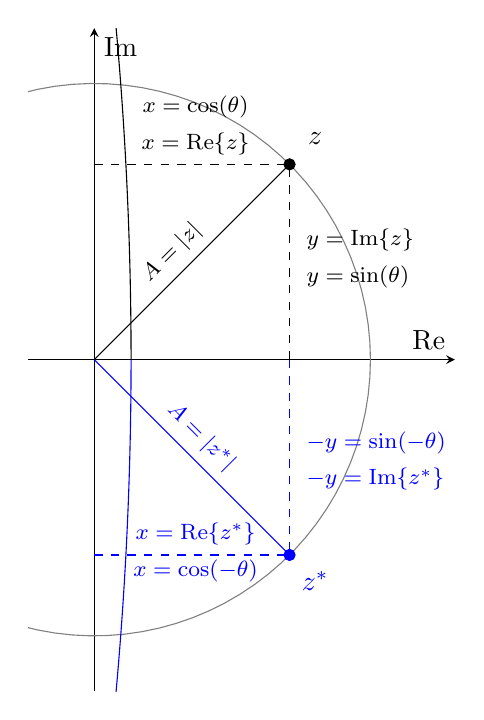
\begin{tikzpicture}
      \begin{axis}[axis equal, ymin=-1.8,xmin=-0.2,ymax=1.8,xmax=1.8,  ticks=none,
          xlabel=$\mathrm{Re}$,
          ylabel=$\mathrm{Im}$, axis lines = center, width=7cm, height=10cm]

        \addplot [gray,domain=0:2*pi,samples=100]({1.5*cos(deg(x))},{1.5*sin(deg(x))});

        \addplot [black, mark = *] coordinates {( {1.5*cos(45)}, {1.5*sin(45)} )} {};
        \addplot [blue, mark = *] coordinates {( {1.5*cos(-45)}, {1.5*sin(-45)} )} {};        
        %   \addplot [black, mark = *] coordinates {( {1.5*cos(-60)}, {1.5*sin(-60)} )} {};   

        \addplot [black] coordinates { (0,0) ( {1.5*cos(45)}, {1.5*sin(45)} ) };

        \addplot [blue] coordinates { (0,0) ( {1.5*cos(-45)}, {1.5*sin(-45)} ) };

        \addplot [dashed,black] coordinates { ({1.5*cos(45)},0) ( {1.5*cos(45)}, {1.5*sin(45)} ) };

        \addplot [dashed,blue] coordinates { ({1.5*cos(45)},0) ( {1.5*cos(45)}, {1.5*sin(-45)} ) };

        \addplot [dashed,black] coordinates { (0,{1.5*sin(45)}) ( {1.5*cos(45)}, {1.5*sin(45)} ) };

        \addplot [dashed,blue] coordinates { (0,{1.5*sin(-45)}) ( {1.5*cos(45)}, {1.5*sin(-45)} ) };

        \draw[draw=black] (axis cs:0.2,0.00) arc [radius={transformdirectionx(0.2)},start angle=0,end angle=45]
        node[midway,right,inner sep=3pt,font={\footnotesize}]{$\theta=\angle z$};

        \draw[draw=blue] (axis cs:0.2,0.00) arc [radius={transformdirectionx(0.2)},start angle=0,end angle=-45]
        node[midway,right,inner sep=3pt,font={\footnotesize}]{{\color{blue}$-\theta=\angle z^*$}};

        \node at (axis cs:0.55,1.06) [above, font={\footnotesize}]{$x=\mathrm{Re}\{z\}$};
        \node at (axis cs:0.55,1.26) [above, font={\footnotesize}]{$x=\cos(\theta)$};        
        \node at (axis cs:0.55,-1.06) [above, font={\footnotesize}]{{\color{blue}$x=\mathrm{Re}\{z^*\}$}};
        \node at (axis cs:0.55,-1.26) [above, font={\footnotesize}]{{\color{blue}$x=\cos(-\theta)$}};                

        \node at (axis cs:1.1,0.65) [right, font={\footnotesize}]{$y=\mathrm{Im}\{z\}$};
        \node at (axis cs:1.1,0.45) [right, font={\footnotesize}]{$y=\sin(\theta)$};        
        \node at (axis cs:1.1,-0.65) [right, color=blue, font={\footnotesize}]{$-y=\mathrm{Im}\{z^*\}$};
        \node at (axis cs:1.1,-0.45) [right, color=blue, font={\footnotesize}]{$-y=\sin(-\theta)$};        

        \node at (axis cs:1.2,1.2) {$z$};
        \node at (axis cs:1.2,-1.2) {{\color{blue}$z^*$}};        

        \node at (axis cs:0.5,0.5) [above,rotate=45,font={\footnotesize}]{$A=|z|$};
        \node at (axis cs:0.5,-0.5) [above,rotate=-45,font={\footnotesize}]{{\color{blue}$A=|z^*|$}};        
      \end{axis}
    \end{tikzpicture}
  \end{center}
  \caption{The polar representation of a complex number $z=x+iy =Ae^{i\theta}$ and its conjugate $z^* = x - iy = A e^{-i\theta}$}
  \label{fig:polar_euler}
\end{marginfigure}

\if 0
  \begin{marginfigure}

    \begin{center}
      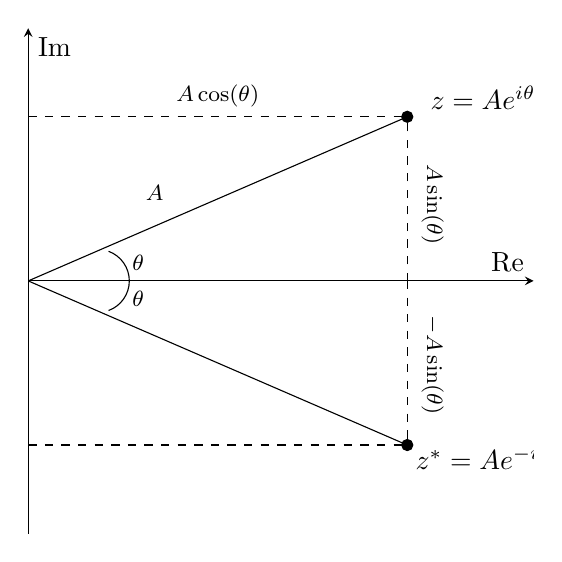
\begin{tikzpicture}
        \begin{axis}[
            ymin=-2.0,
            xmin=0.0,
            ymax=2.0,
            xmax=1.0,
            ticks=none,
            xlabel=$\mathrm{Re}$,
            ylabel=$\mathrm{Im}$,
            axis lines = center,
            width=8cm, height=8cm]
          \addplot [black, mark = *] coordinates {( {1.5*cos(60)}, {1.5*sin(60)} )} {};
          \addplot [black, mark = *] coordinates {( {1.5*cos(-60)}, {1.5*sin(-60)} )} {};

          \addplot [black] coordinates { (0,0) ( {1.5*cos(60)}, {1.5*sin(60)} ) };
          \addplot [dashed,black] coordinates { ({1.5*cos(60)},0) ( {1.5*cos(60)}, {1.5*sin(60)} ) };
          \addplot [dashed,black] coordinates { (0,{1.5*sin(60)}) ( {1.5*cos(60)}, {1.5*sin(60)} ) };

          \addplot [black] coordinates { (0,0) ( {1.5*cos(-60)}, {1.5*sin(-60)} ) };
          \addplot [dashed,black] coordinates { ({1.5*cos(-60)},0) ( {1.5*cos(-60)}, {1.5*sin(-60)} ) };
          \addplot [dashed,black] coordinates { (0,{1.5*sin(-60)}) ( {1.5*cos(-60)}, {1.5*sin(-60)} ) };

          %  \draw [black,-] (0,0) arc [radius=0.5,start angle=0,end angle=60];
          \draw[draw=black] (axis cs:0.2,0) arc [radius=0.4cm,start angle=0,end angle=70]
          node[midway,right,inner sep=3pt,font={\footnotesize}]{$\theta$};

          \draw[draw=black] (axis cs:0.2,0) arc [radius=0.4cm,start angle=0,end angle=-70]
          node[midway,right,inner sep=3pt,font={\footnotesize}]{$\theta$};

          \node at (axis cs:0.375,1.3) [above, font={\footnotesize}]{$A\cos(\theta)$};
          \node at (axis cs:0.8,1.0) [right, rotate=-90, font={\footnotesize}]{$A\sin(\theta)$};
          \node at (axis cs:0.8,-0.20) [right, rotate=-90, font={\footnotesize}]{$-A\sin(\theta)$};

          \node at (axis cs:0.9,1.45) {$z= A e^{i\theta}$};
          \node at (axis cs:0.9,-1.4) {$z^* = A e^{-i\theta}$};
          \node at (axis cs:0.25,0.7) [font={\footnotesize}]{$A$};

        \end{axis}
      \end{tikzpicture}
    \end{center}
    \caption{A complex number $z=x+iy =Ae^{i\theta}$, and it's complex conjugate $z^* = x-iy = A e^{-i\theta}$.}
    \label{fig:conjugate}
  \end{marginfigure}
\fi
% complex numbers

\newthought{\index{Euler's formula}{Euler's formula} relates an arbitrary \index{complex
  number}{complex
  number} $z \in \mathbb{C}$ to an exponential function of the \index{natural
  number}{natural
  number} $e$} and the $\sin$ and $\cos$ trigonometric functions as follows:
\begin{equation}
  \boxed{
    z = x + iy = A e^{i\theta} = A[\cos(\theta)+i\sin(\theta)]
  }\,\,.
  \label{eq:eulerintro}
\end{equation}
This formula is useful, as it provides a relationship between the Cartesian and \index{polar representation}{polar representation} of a \index{complex number}{complex number}\footnote{The \emph{\index{proof of Euler's formula}{proof of Euler's formula}} can be obtained in several different ways. We will use the derivative method demonstrated out by Youtuber MichaelPennMath. It relies on investigating that $f(\theta)=e^{-i\theta}e^{i\theta}=1$ holds when $e^{i\theta}=cos\theta + i\sin\theta$. Consider the following function:
\[
f(\theta) = e^{-i\theta}[\cos(\theta)+i\sin(\theta)].
\]
We know that $f(0)=1$ just by relying on $e^0=0$, $\cos(0)=1$ and $\sin(0)=0$. The derivative of this function is zero everywhere:
\begin{align*}
\frac{df}{d\theta} =& e^{-i\theta}[-\sin(\theta)+i\cos(\theta)] \\
&- i e^{-i\theta}[\cos(\theta)+i\sin(\theta)] \\
= & 0
\end{align*}
From this, we know that $f(\theta) = f(0) = 1$. The function is constant everywhere.

With a little bit of algebra, we can see that because $f(\theta)=1$, then $e^{i\theta}=e^{i\theta} f(\theta)$, and thus
\[
e^{i\theta} = \cos(\theta) + i\sin(\theta).
\]
This proves Euler's formula.}.



In this formula, $A = |z|=\sqrt{x^2 + y^2}$ is the absolute value of the complex number $z$. This is sometimes called the \emph{\index{magnitude}{magnitude}} or
\emph{\index{modulus}{modulus}} of $z$.

The angle $\theta$ can be obtained with simple geometry
$\theta=\tan^{-1}(y/x)$. The angle is also sometimes called the \emph{\index{argument}{argument}} of $z$. We'll use the following notation to denote the argument of a complex number: $\angle z = \theta = \tan^{-1}(y/x)$. In some other texts you might run into the following notation: $\angle z = \mathrm{Arg\{z\}}$.

It is worth pointing out here is that it is possible to add an integer
multiple of $2\pi$ to $\theta$ and still get the same complex number:
\begin{equation}
  A e^{i\theta} = A e^{i(\theta + 2\pi k)}
\end{equation}
This is due to the fact that $e^{i2\pi k} = 1$, where
$k \in \mathbb{Z}$ is an arbitrary integer. The fact that there are
infinitely many different solutions to the argument of a complex
number is an important property, which will be encountered often in
signal processing. For example, the concept
of \emph{\index{aliasing}{aliasing}} of discretized signals, which will
encounter later on, occurs due to this this property.

The term $i$ in Equation \ref{eq:eulerintro} is the imaginary number, which has the following properties: $i=\sqrt{-1}$ and $i^2 = -1$. In engineering and programming, the symbol $j$ is also often used for the imaginary number instead of $i$. The Python programming language uses the symbol $j$, and to denote e.g., $z=2+5i$ in Python, you would use the code snippet \verb|z=2+5j|.   % I'll use $i$, but you can use whichever notation you prefer yourself.

The geometric representation of a complex number is shown in
Figure \ref{fig:polar_euler}, which shows the real and imaginary
components of a complex number in a two-dimensional coordinate system-- the complex plane.

The complex exponential obey the same exponentiation rules as the real exponential function:
\begin{equation}
  \boxed{
  e^{z_{1}}e^{z_{2}} = e^{z_{1}+z_{2}}
  }\,\,.
  \label{eq:complexexponentiation}
\end{equation}
for all complex numbers $z_{1},z_{2}\in\mathbb{C}$, moreover $(e^{z_{1}})^{z_{2}}=e^{z_{1}z_{2}}$.

\newthought{The conjugate $z^*$} of complex number $z$ is defined as:
\begin{align}
  z^* & = x - iy                         \\
      & =A[\cos(\theta)-i\sin(\theta)]   \\
      & =A[\cos(-\theta)+i\sin(-\theta)] \\
      & =A e^{-i\theta}\,\,.
\end{align}
The conjugation operation flips the sign of the imaginary
component. The geometric interpretation of the \index{complex conjugate}{complex conjugate} is
shown in Figure \ref{fig:polar_euler}.  We'll use the superscript star notation to denote the conjugation operator.

\newthought{The complex conjugate can be used to obtain the magnitude of the complex number}:
\begin{equation}
\boxed{
|z| = \sqrt{z z^*} = \sqrt{x^2 + y^2}.
}
\end{equation}
%as $zz^*=(x+iy)(x-iy)=x^2+y^2$
%or $zz^* = |z|e^{i\theta}|z|e^{-i\theta}=|z|^2$.

\newthought{A complex conjugate can also be used to select the real and imaginary
  components of a complex number} as follows:
\begin{equation}
\boxed{
  \Re{z}  = \frac{1}{2}(z+z^*)=x
  \label{eq_conj}
  }
\end{equation}
and 
  \begin{equation}
\boxed{
  \Im{z}  = \frac{1}{2i}(z-z^*)=y
  \label{eq_conj2}
  }
\end{equation}
These formulas are often encountered when dealing with real-valued signals. It is often easier to algebraically to manipulate signals of the form $Ae^{i\theta}$, and after the calculations are done, it is simply a matter of using equation \ref{eq_conj} to extract the real component of the signal from its complex representation. 

\newthought{The use of a sum of a complex number and it's conjugate can be used to relate the exponent function to a cosine and sine function}. Using Euler's formula for $z=e^{i\theta}$ and Equations \ref{eq_conj} and \ref{eq_conj2}, we can obtain:
\begin{equation}
\boxed{
  \cos(\theta)  = \frac{1}{2}\left(e^{i\theta} + e^{-i\theta}\right) \label{inveul0}
  }
  \end{equation}
\begin{equation}
\boxed{
  \sin(\theta)  = \frac{1}{2i}\left(e^{i\theta} - e^{-i\theta}\right). \label{inveul}
  }
\end{equation}
These relations are sometimes called the \emph{\index{inverse
    Euler}{inverse Euler}} relations. You'll encounter these formulas when converting a $\cos$ or $\sin$ function into two complex exponent functions. The first step of a signal processing related calculation involving real-valued signals is often making this conversion, as functions of the form $A e^{i\theta}$ are significantly easier to deal with.

\begin{marginfigure}
  \begin{center}
\includegraphics[width=\textwidth]{ch03/figures/compmult.png}
\end{center}
  \caption{Multiplication of two complex numbers (TBD: cleanup figure)}
  \label{fig:comp_mult}
\end{marginfigure}

\newthought{Complex multiplication can be viewed as multiplication of magnitudes and summation of phases}. Let's express two complex numbers in polar form as $z_1=A_1e^{i\theta_1}$ and $z_2=A_2e^{i\theta_2}$. We can now see that multiplication with complex numbers has an intuitive interpretation.
\begin{equation}
  z_1 z_2 = A_1 e^{i\theta_1} A_2 e^{i\theta_2} = \underbrace{A_1
    A_2}_{A_3} \underbrace{e^{i(\theta_1 + \theta_2)}}_{e^{i\theta_3}} =
  A_3 e^{i\theta_3} \,\,.
\end{equation}
When multiplying two numbers, the resulting angle is a sum of the two angles $\theta_3=\theta_1 + \theta_2$, which can be also seen as a rotation of the point indicated by a complex number $z_1$ by angle $\theta_2$ on the complex plane. The new magnitude is the magnitudes of the two numbers multiplied together $A_3=A_1A_2$. Figure \ref{fig:comp_mult} demonstrates multiplication geometrically on the complex plane.

\begin{figure}
  \begin{center}
    \includegraphics[width=\textwidth]{code/006_spiral/spiral.png}
  \end{center}
  \caption{A spiral is formed by evaluating $z^n$ with integer values of $n$ between $0$ and $41$. In this case $z = 0.92 e^{i 2\pi /20}$. The parametric curve $e^{i\theta}$ with $\theta \in \mathbb{R}$ draws a circle in the complex plane, which is depicted with a gray color. The code that generated this plot can be found in \texttt{006\_spiral/spiral.py}.}
  \label{fig:spirals}
\end{figure}

\newthought{Raising a complex number to the $n$th power} can be seen as exponential scaling and rotation. Consider a complex number
\begin{equation}
  z = A e^{i\theta}
\end{equation}
where $A \in \mathbb{R}_{\ge 0}$ and $\theta \in \mathbb{R}$. If we raise this to the $n$th power, we get:
\begin{equation}
  z^n = A^n e^{i\theta n} = A^n [\cos(\theta n) + i \sin(\theta n)]\,\,.
\end{equation}
Scaling and rotation is demonstrated in Figure \ref{fig:spirals}.

\newthought{Here are some Python examples of complex number operations}.

\lstinputlisting[language=Python, caption={\texttt{008\_complex\_ops/ops\_example.py}}, label=lst:ex1]{code/008_complex_ops/ops_example.py}





\newpage
\section{Exercises: Complex Algebra}

\begin{enumerate}
\item Prove $e^{i\pi}+1=0$ using Euler's formula. 
\item Use Euler's formula to write $1/i$ into polar form $Ae^{i\phi}$. What is the phase angle $\phi$?
\item Show that $i^{i}$ is real valued using Euler's formula. 
\item Use Euler's formula to show that de Moivre's formula is valid for $n\in\mathbb{Z}$:
$$[\cos(x)+i\sin(x)]^{n}=\cos(nx)+i\sin(nx)$$

\item Using Euler's formula, it is possible to determine the $n$th root of unity. What this means is that we look for all unique values of $z$ which satisfy the following equation where $n$ is a positive integer:
\begin{equation}
    z^{n}=1.
    \label{ch03:eq_unity}
\end{equation}
You probably already know the answer in the case of $n=2$, for which there are two solutions: $z_{0}=1$ and $z_{1}=-1$ as both $1^{2}=1$ and $(-1)^{2}=1$. \\
Provide a general formula that gives $n$ unique values of $z$ that
satisfy Equation \ref{ch03:eq_unity}. How many unique solutions of $z$ are there
for each value of $n$? Hint: remember that $e^{i 2\pi k} = 1$ where
$k$ is an integer. 
\item Use the inverse Euler formula to convert $(1-i) e^{-i \omega t} + (1+i) e^{i
  \omega t}$ into the following form:
\begin{equation*}
    A \cos(\omega t  + \phi)
\end{equation*}
with $A\in \mathbb{R}$. What is $A$ and what is $\phi$?

\item Prove using Euler's formula that:
\begin{equation*}
    \cos(3\theta )= \cos^3(\theta)-3\cos(\theta)\sin^2(\theta).
\end{equation*}

\item Use Euler's formula to prove the following trigonometric identity:
\begin{align*}
\cos(\alpha + \beta)&=\cos(\alpha)\cos(\beta) - \sin(\alpha)\sin(\beta)\,\,.
\end{align*}

\item Another definition of $e^{z}$ (the complex exponential) is by an extension of the Taylor series expansion of $e^{x}$ (the real exponential) as follows
$$e^{z}:=\sum_{k=0}^{\infty}\frac{z^{k}}{k!}, \quad\quad \text{for}\ z\in\mathbb{C}.$$
That is, $e^{z}$ is taken to mean this infinite series. Use this Taylor series expansion definition to show that
\begin{equation}
  e^{i\theta} = \cos(\theta) + i\sin(\theta).
  \label{ch03:euler_formula}
\end{equation}
To do this, compute the Taylor series expansion of $e^{i\theta}$. 

\end{enumerate}
\fi

\ifSpSigSys
\chapter{Signals and Systems}
% what is a signal and what is a system?
%
% introduces:
% - signal
% - continuous-time and discrete-time signal
% - dependent and independent variable
% - system
%
\newthought{What is a signal and what is a system?} By
a \emph{\index{signal}{signal}}, we mean an information carrying mathematical function. Any function that has a value as a function of one or more variables is in essence a signal. 
By a \emph{\index{system}{system}}, we denote a mathematical operation that modifies a signal. A system consists of the precise mathematical description of how a signal fed into a system is modified by the system to produce an output signal.

The definition of signals and systems are merely abstract concepts, which have gained acceptance in the engineering community. In the context of mathematics, signals could also be called functions or vectors. 
Systems would be called functions or operators. In computer science, signals are often treated as arrays of numbers in the memory of a computer and systems are algorithms and computer programs that operate on these arrays.

\section{Signals}
\index{signal}

\begin{marginfigure}%
\begin{center}
\begin{tikzpicture}
\begin{axis}[width=\textwidth,
	xticklabels=\empty,
	yticklabels=\empty,		
	xmin=-1.5,xmax=6,
	axis x line=bottom,
	axis y line=left,
	xlabel={Independent variable $t$},
	xlabel style={below},
	ylabel={Dependent variable $x(t)$},
    xlabel style={ yshift = { 1em } },
    ylabel style={ yshift = { -2.2em } }
]
\addplot[draw=blue,domain=-1:7,samples=150] {(x>0)*exp(-x)};
\end{axis}
\end{tikzpicture}
\end{center}
\caption{Continuous-time signal.}
\label{fig:ctfig}
\end{marginfigure}

\begin{marginfigure}%
\begin{center}
\begin{tikzpicture}
\begin{axis}[width=\textwidth,
%	title={Discrete-time signal},
	xticklabels=\empty,
	yticklabels=\empty,	
	xmin=-1.5,xmax=6,
	axis x line=bottom,
	axis y line=left,
	xlabel={Independent variable $n$},
	xlabel style={below},
	ylabel={Dependent variable $x[n]$},
    xlabel style={ yshift = { 1em } },
    ylabel style={ yshift = { -2.2em } }
]
\addplot+[ycomb,domain=-1:5,samples=15] {(x>0)*exp(-x)};
\end{axis}
\end{tikzpicture}
\end{center}
\caption{Discrete-time signal.}
\label{fig:dtfig}
\end{marginfigure}


\newthought{A \index{signal}{signal}} is a mathematical function $x(t)$, which describes the value of a \index{dependent variable} dependent variable $x$, as a function of an \index{independent variable}independent variable $t$. An independent variable ``sweeps'' through all possible values. The dependent variable is the variable that changes as a function of the independent variable and conveys information.

Here's an example. When describing electric potential as a function of time $V(t)$, time $t$ is the independent variable and the electric potential $V(t)$ as a function of time is the dependent variable. Time by itself does not convey information, but electric potential as a function of time does.

Physical ``real world'' signals are modeled as continuous-time signals. Examples include, amongst countless others:
\begin{itemize}
 \setlength\itemsep{0.25em}        
\item temperature,
\item density,
\item pressure as a function of time and space (sound, seismic waves),
\item electric field as a function of time and position
  (electromagnetic waves), or
\item electrical current in a circuit.
\end{itemize}
Physics relies on differential calculus, with integration and differentiation as elementary operators. As we will later see, differential calculus can be studied through methods of signal processing, especially the spectral techniques and the Fourier transform are useful tools that can be applied in differential calculus.

This course will focus primarily on one-dimensional signals. These signals are complex valued functions $x(t) \in \mathbb{C}$ of a real valued argument $t\in \mathbb{R}$. This will naturally also cover the
special case, where the signal is real-valued
$x(t) \in \mathbb{R} \subset\mathbb{C}$. 

By convention, we will refer to the independent variable of a signal as time, even though this variable doesn't necessarily have to indicate time. It can represent anything. For example, the independent variable can just as well be, e.g., distance.

Signals can be continuous or discrete. Following a commonly adopted practice, we will use round brackets for continuous-time signals (e.g., $x(t)$) and square brackets for discrete-time signals (e.g., $x[n]$). 

In the case of discrete-time signals, the sample index
$n \in \mathbb{Z}$ is unitless. A discrete-time signal is merely a sequence of numbers. The only way to associate meaning to this sequence of numbers is the a priori knowledge of how the signal was discretized. This allows us to, e.g., map the $n$th sample to a real valued time.

An example of a continuous-time and a discrete-time signal is shown in Figures \ref{fig:ctfig} and \ref{fig:dtfig}. When plotting signals graphically, it is customary (but not mandatory) to use the horizontal axis for the independent variable, and the dependent variable on the vertical axis.

To summarize, the two main types of signals that this course deals with are one-dimensional continuous-time $x(t)$ and one-dimensional discrete-time signals $x[n]$. Continuous-time signals are mappings from the real axis (time) to the set of complex numbers:
\begin{equation}
\boxed{
x: \mathbb{R} \rightarrow \mathbb{C}
}
\end{equation}
Discrete-time signals are mappings from the set of integers to the set of complex numbers:
\begin{equation}
\boxed{
x: \mathbb{Z} \rightarrow \mathbb{C}
}
\end{equation}
Signal processing of higher dimensional signals are essentially functions of the form
\begin{equation}
x: \mathbb{R}^N \rightarrow \mathbb{C}
\end{equation}
or in the case of discrete-time:
\begin{equation}
x: \mathbb{Z}^N \rightarrow \mathbb{C}
\end{equation}

\newthought{The first experimental detection of gravitational waves} using the Laser Inteferometer Gravitational-Wave Observatory (LIGO) is shown in Figure \ref{fig:ligo_meas}. This signal is an example of a one-dimensional signal. The signal is thought to be caused by two black holes with masses around 30 solar masses merging together, 1.3 billion light-years from Earth. The independent variable on the x-axis is time, and the dependent variable is strain (stretching) of space that occurs due to a gravitational wave passing through the instrument. This is measured by comparing the relative lengths of two 4 km long laser interferometer arms. 

\begin{figure}
\begin{center}
\includegraphics[width=\textwidth]{ch04/figures/dc_fg.png}
\end{center}
\caption{Two independent one dimensional signals measured by LIGO depicting strain. This is stretching of space due to a gravitational wave passing through two geographically separated laser interferometer observatories. One in Hanford, WA (left), and one in Livingston, LA (right). The figure is from: B. P. Abbott et al. (LIGO Scientific Collaboration and Virgo Collaboration) Phys. Rev. Lett. 116, 061102 – Published 11
February 2016.}
\label{fig:ligo_meas}
\end{figure}

\newthought{Signals can be of arbitrary dimension}. For example, an image is a 2d signal, where the dependent variable is intensity $I(x,y)$ measured as a function of two independent spatial variables $x$ and $y$ that indicate distance from origin along two orthogonal axes.  An example of a discrete-time two-dimensional signal is shown in Figure \ref{fig:bh_example}. 
It represents an image of the emission from hot gas in the event horizon of a black hole around the M87 galaxy. 
The image is obtained using a technique called very long baseline interferometry, which utilizes measurements from radio telescopes around the world. 
These measurements are combined to simulate a large telescope with the resolution equivalent to a telescope approximately the size of Earth.\footnote{The Fourier transform, which is one of the central themes in this course, is a key part of the mathematics of very long baseline interferometric imaging.}

Even higher dimensional signals can be used. Consider for example a video. It is a signal that contains the intensity of an image as a function of time. You can think of a moving picture (movie) as a three-dimensional signal: $I(x,y,t)$, where the intensity of the image is a function of two-dimensional position as well as time.

While we will focus primarily on one dimensional signals in order to keep things simple, many of the concepts we discuss can be generalized to multiple dimensions. 
Two-dimensional signal processing is called image processing, and it shares many of the same basic concepts with one dimensional signal processing. 
I will try to occasionally give examples of signal processing with higher dimensional signals.

%\begin{figure}
%\begin{center}
%\includegraphics[width=\textwidth]{ch01/2dsig.png}
%\end{center}
%\label{fig:2dexim}
%\caption{An example of a 2d signal: 32-cm wavelength opposite
%  circularly polarized inverse synthetic aperture radar map of the
%  Moon, obtained using the EISCAT radar in Troms\o{}. Image intensity
%  represents backscattered power from the surface of the Moon.}
%\end{figure}

\begin{figure}
\begin{center}
\includegraphics[width=0.68\textwidth]{code/004_dft_2d/bhi.png}
\end{center}
\caption{An example of a 2d signal: A Very Long Baseline Interferometric radio image of
the black hole at the center of galaxy M87. The intensity depicts what is thought to be hot gas outside the event horizon of the black hole. Credit: Event Horizon Telescope collaboration et al. 2019.}
\label{fig:bh_example}
\end{figure}

\newthought{Digital signals} on a computer, are also quantized. This means that there is only a finite number of possible values for the dependent value of a signal. 
This type of signal is called a \emph{\index{quantized}{quantized}} signal. We will not discuss quantization in this course.


\section{Systems}
%\newcommand{\sign}{\text{sign}}

\newthought{A signal processing \index{system}{system}} can be represented graphically as a block diagram, which describes signals going into a system, and signals going out of a system. 
An example is shown in Figure \ref{simple_sps}

\begin{figure}
\tikzstyle{int}=[draw]
%\tikzstyle{init} = [pin edge={to-,thin,black}]
\tikzstyle{init} = []
% [pin edge={to-,thin,black}]

\begin{center}
  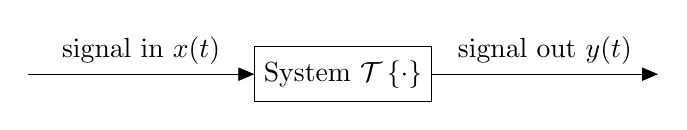
\begin{tikzpicture}[node distance=4cm,auto,line width=0.1mm,>=triangle 45]
    \node [int] (a) {System $\spop$};
    \node (b) [left of=a,node distance=4cm, coordinate] {a};
    %\node [int, pin={[init]above:$p_0$}] (c) [right of=a] {$\frac{1}{s}$};
    \node [coordinate] (end) [right of=a, node distance=4cm]{};
    \path[->] (b) edge node {signal in $x(t)$} (a);
    %\path[->] (a) edge node {$v$} (c);
    \draw[->] (a) edge node {signal out $y(t)$} (end) ;
\end{tikzpicture}
\end{center}
\label{simple_sps}
\caption{A simple signal processing system block diagram.}
\end{figure}
A graphical representation is useful for understanding a signal processing system, especially if it is a complicated one, which includes many systems and signals.

The following block diagram is a real-world example of the block diagram of the EISCAT Svalbard radar transmitter subsystem. 
\begin{figure}
\begin{center}
\includegraphics[width=\textwidth]{ch04/figures/wannberg97.jpg}
\end{center}
\caption{An example of a more complicated block diagram. From: Wannberg et.al., 1997.}
\label{fig:esr}
\end{figure}

The mathematical description of a system (what goes on in the box) is a general transformation of a signal. 
The mathematical notation for a continuous-time system in general is\footnote{Here $\spop$ is a mathematical description of how the input signal is modified by the signal processing system. This is also called an
\index{operator}{operator}}:
\begin{equation}
\boxed{
y(t) = \spop[x(t)]
}
\end{equation}
and for discrete-time system:
\begin{equation}
\boxed{
y[n] = \spopb\{x[n]\}
}
\end{equation}
An example of a system could be a function that delays the input
signal by a delay $\tau$:
\begin{equation}
y(t) = x(t-\tau).
\end{equation}
Another example is a linear amplifier, which multiplies the amplitude
of the signal with a constant $\alpha \in \mathbb{C}$:
\begin{equation}
y(t) = \alpha x(t).
\end{equation}
You will often encounter both of these types of systems.

\newthought{For example, we can use these two basic systems to make a simplified model of a radar}. Imagine that you have a radar. This radar sends out a waveform that is described by a waveform $x(t)$. Let's say that the
time it takes an electromagnetic wave to travel from the radar transmitter to a point-like radar target and back is $\tau$ seconds. The received radar echo will be a delayed version of the transmitted signal, which is delayed by $\tau$. In addition to this, the signal will be scaled, as a radar echo is typically much weaker than the transmitted signal.

Therefore, a very simple system that describes a radar echo is the following:
\begin{equation}
y(t) = \alpha x(t-\tau)
\end{equation}
where $y(t)$ is the received radar echo signal.

We can further expand this concept to write the equation that describes a radar echo for a situation where there can be a continuous radar echo at time delays between $0$ and $T$:
\begin{equation}
y(t) = \int_0^T \alpha(\tau) x(t-\tau) d\tau.
\end{equation}
In this case, $\alpha(\tau)$ describes the radar echo amplitude as a function of propagation delay. This type of equation is called a \emph{\index{convolution}convolution} equation. 
You will encounter this type of equation very often in signal processing, and find that the Fourier transform is a very useful tool when dealing with convolution equations.

\newthought{Differential operators can also be seen as
systems}. Consider the first time-derivative of the continuous-time signal $x(t)$:
\begin{equation}
y(t) = \frac{d}{d t}x(t).
\end{equation}
The system definition is the time derivative operator $\frac{d}{dt}$.

\newthought{Systems are classified based on their mathematical properties}. The most important two are: \emph{\index{linearity}{linearity}} and \emph{\index{time-invariance}{time-invariance}}. A
system which is both linear and time-invariant is called 
\index{linear time-invariant}{linear time-invariant} 
(LTI)\index{LTI}. Such systems have beneficial mathematical properties that make analysis and design of such systems very straightforward. 
We'll later on prove that LTI systems are fully characterized by something known as an impulse response. This is an important concept in signal processing.

\section{Linear system}
\index{Linear system}

\begin{marginfigure}[-3cm]
\tikzstyle{int}=[draw, minimum size=2em]
\tikzstyle{init} = [pin edge={to-,thin,black}]

\begin{center}
% Definition of blocks:
\tikzset{%
  block/.style    = {draw, thick, rectangle, minimum height = 3em,
    minimum width = 3em},
  sum/.style      = {draw, circle, node distance = 2cm}, % Adder
  input/.style    = {coordinate}, % Input
  output/.style   = {coordinate} % Output
}
% Defining string as labels of certain blocks.
\newcommand{\suma}{\Large$+$}
\newcommand{\inte}{$\displaystyle \int$}
\newcommand{\derv}{\huge$\frac{d}{dt}$}
\newcommand{\mula}{\Large$\cross$}

\begin{tikzpicture}[auto, line width=0.1mm, node distance=2cm, >=triangle 45]
% make an op block
\draw 
   node at (0,0) [block, name=op0] {$\spop$};
% make a sum block
\draw 
   node at (-1.5,0) [sum, name=suma2] {\suma};
% output node
\draw 
   node at (1.5,0) [name=out0] {$y_1(t)$};

% input node 1
\draw 
   node at (-3,1.5) [name=in0] {$x_1(t)$};

% input node 2
\draw 
   node at (-3,-1.5) [name=in1] {$x_2(t)$};

% make a mult block
\draw 
   node at (-1.5,1.5) [sum, name=mul0] {\mula};
% make a mult block
\draw 
   node at (-1.5,-1.5) [sum, name=mul1] {\mula};

% output node
\draw 
   node at (0,1.5) [name=c0] {$c_2$};

% output node
\draw 
   node at (0,-1.5) [name=c1] {$c_1$};
% join
\draw[->](suma2) -- node {}(op0);
\draw[->](mul0) -- node {}(suma2);
\draw[->](mul1) -- node {}(suma2);
\draw[->](op0) -- node {}(out0);
\draw[->](in0) -- node {}(mul0);
\draw[->](in1) -- node {}(mul1);
\draw[->](c0) -- node {}(mul0);
\draw[->](c1) -- node {}(mul1);
\end{tikzpicture}

\vspace{1em}
\begin{tikzpicture}[auto, line width=0.1mm, node distance=2cm, >=triangle 45]
% make an op block
\draw 
   node at (-1.5,1.5) [block, name=op0] {$\spop$};
\draw 
   node at (-1.5,-1.5) [block, name=op1] {$\spop$};
% make a sum block
\draw 
   node at (0,0) [sum, name=suma2] {\suma};
% make a mult block
\draw 
   node at (0,1.5) [sum, name=mul0] {\mula};
% make a mult block
\draw 
   node at (0,-1.5) [sum, name=mul1] {\mula};
% output node
\draw 
   node at (1.5,0) [name=out0] {$y_2(t)$};
% output node
\draw 
   node at (1.5,1.5) [name=c0] {$c_2$};
% output node
\draw 
   node at (1.5,-1.5) [name=c1] {$c_1$};
% input node 1
\draw 
   node at (-3,1.5) [name=in0] {$x_1(t)$};
% input node 2
\draw 
   node at (-3,-1.5) [name=in1] {$x_2(t)$};
% join
\draw[->](suma2) -- node {}(out0);

\draw[->](in0) -- node {}(op0);
\draw[->](in1) -- node {}(op1);

\draw[->](op0) -- node {}(mul0);
\draw[->](op1) -- node {}(mul1);
\draw[->](mul0) -- node {}(suma2);
\draw[->](mul1) -- node {}(suma2);
\draw[->](c0) -- node {}(mul0);
\draw[->](c1) -- node {}(mul1);

\end{tikzpicture}
\end{center}
\label{fig:linearity_block}
\caption{In order for the system specified by $\spop$ to be linear, $y_1(t) = y_2(t)$ must be satisfied.}
\end{marginfigure}

A system is linear, if a linear combination of inputs fed into the system yields the same as the linear combination of outputs:
\begin{equation}
\boxed{
\spop[c_1 x_1(t) + c_2 x_2(t)] = c_1 \spop[x_1(t)] + c_2 \spop[ x_2(t) ]}
\label{def:linear_sys}
\end{equation}
for arbitrary constants $c_1 \in \mathbb{C}$ and $c_2 \in \mathbb{C}$ and arbitrary input signals $x_1(t)$ and $x_2(t)$. This property is highly useful, and appears throughout signal processing.

\newthought{An example of a linear system} is a system that scales the input signal by a constant factor $\alpha$:
\begin{equation}
  y(t) = \alpha x(t).
\end{equation}
If $|\alpha| >1$, the signal is amplified. This type of system would typically be called an amplifier. If $0<|\alpha|<1$, the system would be called an attenuator, as the output signal amplitude would be attenuated.

It is quite easy to determine that the test for linearity is passed for this system:
\begin{equation}
\alpha [c_1 x_1(t) + c_2 x_2(t)] = c_1 [\alpha x_1(t)] + c_2 [\alpha x_2(t)].
\end{equation}

\newthought{An example of a non-linear system} is the following system, which obtains the absolute value of $x(t)$:
\begin{equation}
y(t) = |x(t)|
\end{equation}
It is quite clear that this does not pass the test for linearity:
\begin{equation}
|c_1 x_1(t) + c_2 x_2(t)| \ne c_1 |x_1(t)| + c_2 |x_2(t)|,
\end{equation}
for all possible values $c_1$, $c_2$, $x_1(t)$, and $x_2(t)$.
\begin{marginfigure}
\tikzstyle{int}=[draw, minimum size=2em]
\tikzstyle{init} = [pin edge={to-,thin,black}]

\begin{center}

% Definition of blocks:
\tikzset{%
  block/.style    = {draw, thick, rectangle, minimum height = 3em,
    minimum width = 3em},
  sum/.style      = {draw, circle, node distance = 2cm}, % Adder
  input/.style    = {coordinate}, % Input
  output/.style   = {coordinate} % Output
}
% Defining string as labels of certain blocks.
\newcommand{\suma}{\Large$+$}
\newcommand{\inte}{$\displaystyle \int$}
\newcommand{\derv}{\huge$\frac{d}{dt}$}
\newcommand{\mula}{\Large$\cross$}

\begin{tikzpicture}[auto, line width=0.1mm, node distance=2cm, >=triangle 45]
% make an op block
\draw  
node at (-1.0,3.0) [name=in0] {$x(t)$};

% make an op block
\draw  
node at (-1.0,1.5) [block, name=op0] {$\spop$};

\draw  
node at (-1.0,0) [block, name=delay0] {$\mathcal{D}\{\cdot\}$};

% output node
\draw 
 node at (-1.0,-1.5) [name=out0] {$y_2(t)$};

% make an op block
\draw  
node at (1.0,3.0) [name=in1] {$x(t)$};

% make an op block
\draw  
node at (1.0,0.0) [block, name=op1] {$\spop$};

\draw  
node at (1.0,1.5) [block, name=delay1] {$\mathcal{D}\{\cdot\}$};

% output node
\draw 
 node at (1.0,-1.5) [name=out1] {$y_1(t)$};

% join
\draw[->](in0) -- node {}(op0);
\draw[->](op0) -- node {}(delay0);
\draw[->](delay0) -- node {}(out0);


% join
\draw[->](in1) -- node {}(delay1);
\draw[->](delay1) -- node {}(op1);
\draw[->](op1) -- node {}(out1);


\end{tikzpicture}
\end{center}
\caption{In order for the system specified by $\spop$ to be time-invariant, $y_1(t) = y_2(t)$ must be satisfied. \label{fig:time_inv_block}}
\end{marginfigure}

\section{Time-invariant system}
\index{Time-invariant}

Let us first define a delay system $\mathcal{D}\{x(t)\} = x(t-\tau)$. Let us assume that the output of a system is $y(t) = \spop[x(t)]$. This system is time-invariant if:
\begin{equation}
\boxed{
\mathcal{T}\{\mathcal{D}\{x(t)\}\} = \mathcal{D}\{\mathcal{T}\{x(t)\}\}
\label{def:timeinv}
}
\end{equation}
In other words, it does not matter if the signal is delayed before or after the system $\mathcal{T}\{\cdot\}$. To check time-invariance, we need to verify Equation \ref{def:timeinv}. 

The test for time-invariance is illustrated as a block diagram in Figure \ref{fig:time_inv_block}. 
If you want, you could think of a time-invariant system as a system that satisfies:
$$[\mathcal{T},\mathcal{D}]x(t)=0,$$
where $[\mathcal{T},\mathcal{D}]=\mathcal{T}\mathcal{D}-\mathcal{D}\mathcal{T}$ is the commutator of two operators. 
Thus, a time-invariant system $\mathcal{T}$ is a system that commutes with the time-delay operator $[\mathcal{T},\mathcal{D}]=0$. 

\newthought{An example of a time-invariant system} is the system that returns the absolute value of the input signal $y(t)=|x(t)|$. We can see this by evaluating:
\begin{align}
\mathcal{T}\{\mathcal{D}\{x(t)\}\} &= \mathcal{T}\{x(t-\tau)\}=|x(t-\tau)|\\
\mathcal{D}\{\mathcal{T}\{x(t)\}\} &= \mathcal{D}\{|x(t)|\}=|x(t-\tau)|
\end{align}
Time-invariance holds as the outputs are equal. It doesn't matter if a time-delay is applied to the signal before or after obtaining the absolute value of the input signal.

\newthought{An example of a case that is not time-invariant} is $y(t) = \mathcal{T}\{x(t)\} = t + x(t)$. We can immediately see that the system directly depends on $t$, not only through, the input. 
The formal test also shows that time-invariance is not met:
\begin{align}
\mathcal{T}\{\mathcal{D}\{x(t)\}\} &= \mathcal{T}\{x(t-\tau)\}=t+x(t-\tau) \\
\mathcal{D}\{\mathcal{T}\{x(t)\}\} &= \mathcal{D}\{t + x(t)\}=(t-\tau)+x(t-\tau)
\end{align}
In this case, $\mathcal{T}\{\mathcal{D}\{x(t)\}\}\neq\mathcal{D}\{\mathcal{T}\{x(t)\}\}$ so the system is not time-invariant.

\section{Example: Overdriven amplifier}
\begin{marginfigure}
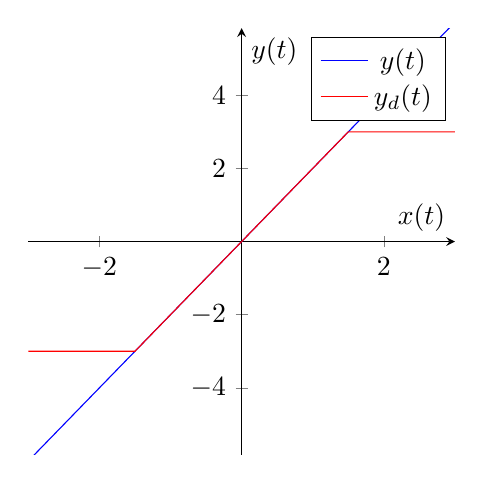
\begin{tikzpicture}
	\begin{axis}[
		xmin=-3, xmax=3,
		height=7cm,
		width=7cm,
		axis x line=center,
		axis y line=center,
                ylabel=$y(t)$,
		xlabel=$x(t)$
	]
		
	\addplot[mark=none,color=blue] {2*x};
	\addlegendentry{$y(t)$}

	\addplot[mark=none,color=red] coordinates {
		(-100,-3)
		(-1.5,-3)
		(1.5,3)
		(100,3)
	};
	\addlegendentry{$y_d(t)$}
	\end{axis}
\end{tikzpicture}
\caption{The system function of a linear amplifier $y(t)$ and a clipping amplifier system $y_d(t)$.}
\label{dist_effect}
\end{marginfigure}

A simple model of a distorted guitar amplifier system would be the
following clipping amplifier system, which is specified as follows:
\begin{equation}
y_d(t) = \left\{
  \begin{array}{rcr}
    -\beta & \mathrm{when} & \alpha x(t)<-\beta \\
    \alpha x(t) & \mathrm{when} & |\alpha x(t)| \le \beta \\
    \beta & \mathrm{when} & \alpha x(t)>\beta 
\end{array}
\right.
\label{clipamp}
\end{equation}
This is a very approximative model of an overdriven guitar
amplifier. This type of system is often encountered in guitar music from the 50s and onwards. I'm sure that once you later implement this in practice, you'll recognize the sound that this system makes.

What does this system do? It amplifies the signal, but only up to a certain point. Beyond a certain absolute value of the input, the output maintains a constant positive or negative value.  This type of behavior is also sometimes called clipping, and the effect is
also sometimes called distortion, as the input signal amplitude is not linearly scaled, but it is rather distorted.

\begin{marginfigure}
  \begin{center}
    \includegraphics[width=\textwidth]{ch04/figures/ampvid.jpg}
  \end{center}
  \caption{A video discussing an overdriven guitar amplifier can be found here: \url{https://youtu.be/I30Mn_-yYF8}.}
\end{marginfigure}
Many real world amplifier systems have this type of saturation behavior. What this often means in practice is that the system is linear when the input absolute amplitude is less than some critical value, but beyond this, linearity no longer holds.

Figure \ref{dist_effect} illustrates what $y_d(t)$ would look like as a function of $x(t)$. It is compared with a normal amplifier system $y(t)=\alpha x(t)$, which does not clip.

\if 0
\begin{center}
\includegraphics[width=0.68\textwidth]{ch01_guitar_amp/clipamp.png}
\end{center}
\fi

\newpage
\section{Exercises: Signals and Systems}
\begin{enumerate}

\item Consider the following signal $V(t)$, which describes the electric potential of a circuit as a function of time. The instantaneous power flowing through this circuit is given by the following equation:
\begin{equation*}
    P(t)=R^{-1}[V(t)]^2.
\end{equation*}
It is possible to consider the function $R^{-1}[\cdot]^2$ that converts electric potential into power as a system in signal processing terminology.
\begin{enumerate}[a)]
\item Is this system linear?
\item Is this system time invariant?
\end{enumerate}
Prove your result.

\item A discrete-time system is defined as:
\begin{equation}
  y[n]= \frac{1}{5}\sum_{k=0}^{4} x[n-k].
\end{equation}
  \begin{enumerate}[a)]
  \item Explain in words what this system does to input signal $x[n]$.
  \item Is this system linear?
  \item Is this system time-invariant?
  \end{enumerate}
Use the tests for linearity and time-invariance to justify your result. 

\item A time scaling system adjusts the scaling of the independent variable: $y(t) = x(\alpha t)$,
when $x(t)$ is the signal fed into the system and $y(t)$ is the output.

\begin{enumerate}[a)]
\item What is the effect on the signal when $0<\alpha<1$?
\item What about $\alpha>1$?
\item Is this system linear?
\item time-invariant?
\end{enumerate}

\item Prove that the time derivative operator $y(t) = \mathcal{T}\{x(t)\} = \frac{d}{dt} x(t)$
is a linear time-invariant system.

\item The following system is defined as the average of the previous
value of the output signal $y[n-1]$ and the current value of the
input signal $x[n]$:
$$y[n]=\frac{1}{2}y[n-1]+\frac{1}{2}x[n].$$
Is this a linear system? In order to show this, you can assume that the input is zero $x[n]=0$ when $n<0$ and that the output $y[n]=0$ when $n=-\infty$. Hint: Try evaluating the value of the values of $y[n]$.

\item The guitar amplifier system given in Equation \ref{clipamp} is not a linear system. Prove this. Hint: you can use proof by example, by finding a case where the requirement of linearity is not met.

\item Is the guitar amplifier system given in Equation \ref{clipamp} a time-invariant system? Prove your result by using the formal test for time-invariance.

\item The code in Listing \ref{lst:audio} implements a linear amplifier system for an audio signal:
\begin{equation}
y(t) = \alpha x(t)
\end{equation}
where the input signal is $x(t)$, the output signal is $y(t)$, and the
amplification is $\alpha$. You can find the code and audio file on
Github.
\lstinputlisting[language=Python,caption={\texttt{003\_guitar/amplifier.py}},label=lst:audio]{ch04/code/amplifier.py}
Run this code and verify that the audio signal stored in
file \verb|guitar_amp.wav| is amplified. You will need to do this by inspecting a before and after amplification plot of the audio signal, as the example code will normalize the amplitude of the signal before storing it to file.

You can use this script as a basis for experimenting with audio signal
processing later on during this course.

\item Change the code in Listing \ref{lst:audio} is such a way that it implements a clipping amplifier as shown in Equation: \ref{clipamp}. Figure out suitable values for $\alpha$ and $\beta$ that make the guitar sound distorted.

\end{enumerate}

\fi



\end{document}